\chapter{A long long road}
Consider an adjective like \data{long}. Repeat it, and its meaning intensifies. That's what The Hollies are doing when they sing:

\begin{quote}
\data{It's a long, long road}\\
\data{From which there is no return}
\end{quote}

\noindent The reduplicative use of \data{long} emphasises the sheer immensity of the journey in a way that the more prosaic \mention{it's a long road} wouldn't.

Another verse, though, goes like this:

\begin{quote}
\data{The road is long}\\
\data{With many a winding turn}
\end{quote}

Now imagine reduplicating \data{long} here. Far from adding emotional depth, it would invite ridicule. As ordinary English, \data{the road is long long} is out. And what's fascinating is that we all intuitively grasp the difference between these two superficially similar uses of repetition. Why? Is there a universal rule at play, or is it something peculiar about the structure of English?

I teach English to international students studying in Canada, some of them beginners, and I've given examples like \data{a long long road} and \data{the road is long long}. There's never any reaction after the first, but laughter inevitably follows the second. The students respond as if they've already learned the boundary.

\bigskip

Before going further, let's pin down what's happening. The phrase \data{a long road} is a noun phrase, where \data{road} is the head noun and \data{long} is an adjective in attributive modifier function, a modifier sitting in front of the noun and ascribing a property to it. \data{The road is long} is a clause. \data{Long} is still an adjective, but here it functions as a predicative complement, the kind that comes after a verb and says something about the subject. Other predicative complements are \data{you're \uline{beautiful}}, \data{they all seem \uline{so happy}}, and \data{I feel \uline{good}}.

The doublet \mention{long long} exemplifies a construction called \term{reduplicative intensification}, \enquote{reduplicative} because the form is repeated and \enquote{intensification} because it pushes the property named by the adjective higher on its scale. The construction is also picky about which adjectives it accepts. \data{Long} is gradable: there are degrees of long. \data{Cambrian}, the geological period, isn't gradable, and *\data{a Cambrian Cambrian fossil} is just as bad as *\data{the road is long long}.

So a more careful statement of what we've seen is this:

\ea[]{In the intensificatory construction, a gradable adjective in attributive modifier function may be repeated to strengthen its meaning. The same pattern isn't generally available when the adjective functions as predicative complement.}\label{def:reduplication-rule}
\z

\section{Same asymmetry, other languages?}

It's tempting to wonder if the pattern repeats in other languages. Japanese has the same asymmetry:

\ea
   \ea[]{
        \gll 長い  長い  道\\
        nagai nagai michi\\
        \glt `a long long road'}
   \ex[*]{
        \gll 道     が 長い 長い\\
        michi ga nagai nagai\\
        \glt `the road is long long'}
   \z
\z

So does Russian:

\ea
    \ea [ ] {
        \gll красивые, красивые глаза\\
        krasivye, krasivye glaza\\
        \glt `beautiful, beautiful eyes'}
    \ex [*] {
        \gll Её глаза красивые, красивые\\
        Yeyo glaza krasivye, krasivye\\
        \glt `her eyes are beautiful beautiful'}
    \z
\z

\noindent Three examples don't establish a rule, but they suggest one. What would such a rule imply?

One answer is universalist: something about the human mind might make intensificatory adjective repetition impossible in predicative function. That answer predicts that no language should allow the construction there.

A second answer is semantic: maybe \mention{long long} means something that works only when the adjective modifies a noun. That answer predicts that the restriction follows from the meaning of the repeated adjective itself.

A third answer is historical: English may simply have developed a construction for repeated adjectives in one position and not another. That answer predicts that other languages may do things differently.

Each answer makes a different prediction.
% EDITORIAL-HPC: This is the cleanest projectibility template in the opening
% movement. Preserve it and later make the payoff explicit: a real grammatical
% account earns its keep by saying what new cases should do, not just by naming
% a rule or mechanism.

\bigskip

% TODO: verify source — Geoff Pullum personal communication suggesting Jamaican Creole; consider footnoting as (Pullum, p.c., YEAR) or absorbing silently.
The universalist hypothesis falls quickly. Jamaican Creole has examples like (\ref{ex:blakblack}).

\ea \label{ex:blakblack}
    \gll\textit{im} \textit{want} \textit{wan} \textit{we} \textit{blakblak}\\
    he wants one that black-black\\
    \glt `he wants one that is very black'\hfill\citep[129]{Gooden2003}.
\z

North-East Ambae, an Oceanic language of Vanuatu, has the same pattern (\ref{ex:qi-qilodo}).

\ea \label{ex:qi-qilodo}
    \gll \textit{Vai-gi} \textit{ngire} \textit{ra=u} \textit{qi-qilodo}\\
        do-become things those short-short \\
    \glt `Those things are very short.'\hfill\citep[278]{Hyslop2004}
\z

\noindent So intensificatory reduplication in predicative position isn't ruled out by anything in the human mind. Some languages permit it. English doesn't.

If it's not a universal of language, where does English's restriction come from?

\section{Old English}

Intensificatory reduplication doesn't seem to have been available in Old English. Two adjectives couldn't really sit side by side modifying a noun directly. *\textit{Micel blæc fugol} `big black bird' would have been unusual; an Old English speaker might have rephrased it as \textit{micel fugol \& blæc} `big bird and black'. But Old English did have a side door: compound nouns. You couldn't put two modifiers in a row, but you could sneak one inside the noun.

\textit{Blackbird} is a Modern English compound, a noun made up of two words: the modifier \textit{black} and the head noun \textit{bird}. \textit{Blackbird} behaves like a single word: its meaning isn't simply \textit{black} plus \textit{bird}, and its internal adjective is hidden from the surrounding grammar. \textit{Really} can modify \textit{black} in \data{a really black bird}, but it can't reach inside to the \textit{black} of *\data{a really blackbird}. Female blackbirds are often brown, and a raven is a black bird, but most certainly not a blackbird.

\begin{figure}
    \centering
    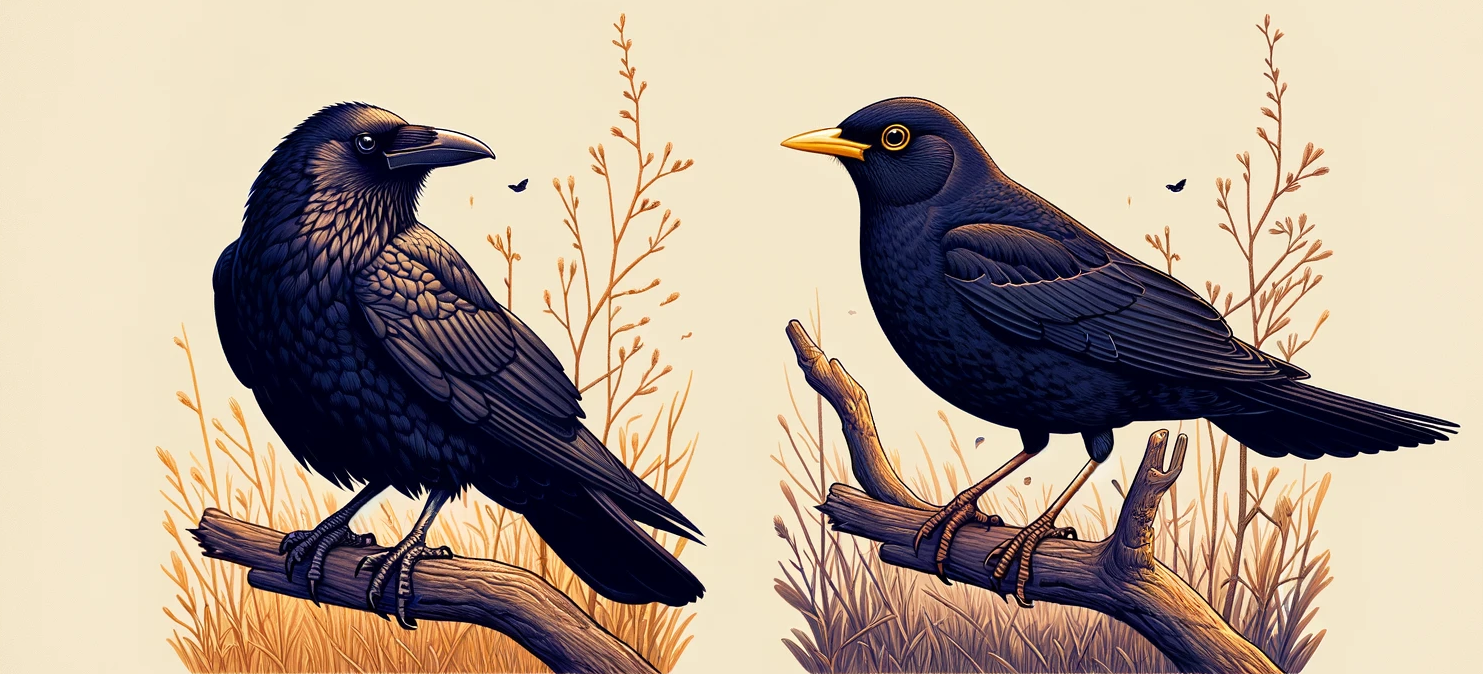
\includegraphics[width=\textwidth]{figures/black-birds.png}
    \caption{A black bird and a blackbird. Image by DALL$\cdot$E.}
    \label{fig:black-birds}
\end{figure}

Although we don't write \mention{citygate} today, \mention{burggeat} was a compound noun in Old English, made up of the modifier \mention{burg} `town/city' and the head noun \mention{geat} `gate'. And just as \mention{really} can't \enquote{see} \mention{black} in \mention{blackbird}, an attributive modifier like \mention{micel} `great' would have been insensitive to \mention{burg} in \mention{burggeat}. With \mention{burg} tucked safely inside the compound noun, \textit{\uline{micel} \uline{burg}geat} wouldn't have felt like two modifiers in a row.

At least, it wouldn't to most speakers. Still, the odd burgher may have interpreted \mention{burggeat} as two words instead of one, and so for them \mention{micel burg geat} would have had two contiguous modifiers. It's only a short step from \mention{micel burg geat} `great city gate' to something like \mention{micel blæc geat} `great black gate' or \mention{fæst eald geat} `strong old gate'. Not only would that have put two modifiers in a row, but both of the modifiers would have been adjectives.

The path to two adjectives is clear when the first half of a compound noun can be mis-parsed as a stand-alone word. But when there's no noun with a modifier to pry loose as a bridge, the path stays closed. That's why English eventually got \data{old old tales}, and never \data{the tale is old old}.

\section{Middle English}

One of the bigger Middle English changes was the erosion of the case system. The Old English forms of \mention{se hring} `the ring' once carried distinct nominative, accusative, genitive, and dative endings. Over time those collapsed into the bare \mention{the ring} and the genitive \mention{the ring's}. As the inflectional endings weakened, word order took on more grammatical work. Without those endings, (\ref{ex:case-loss}) looks like the woman gave the queen a ring; with them, we can see that the queen was the subject and it was \mention{to} the woman that she gave the ring.

\ea \label{ex:case-loss}
    \gll \textit{Þām wife} \textit{sealde} \textit{sēo cwēn} \textit{hring}\\
        {the woman-DAT} gave {the queen-NOM} ring-ACC\\
    \glt `It was to the woman that the queen gave a ring.'
\z

For our purposes, what matters here is the growing stability of positions within the noun phrase that came with the loss of case. With the pre-nominal zone increasingly fixed as the place where modifier material lived, there was room for more of it to accumulate.

That laid the groundwork for a new kind of intensification: near-synonymous adjective stacking, as in (\ref{ex:gosefoote}), with minor spelling adjustments \citep{Gonzalez-Diaz2021}.

% TODO: verify source — Bullein 1579 quotation; no bib entry Bullein1579; verify text and add bibliography entry.
\ea[]{\textit{gosefoote an evill herbe: it is called pes anserinus, leaved like night shade, but more jagged in the said leaves, bearing \ob \uline{small little} red flowers, with great plenty of seede, lyke unto arage\cb.}\\ \hfill (Bulleins bulwarke of defence against all sicknesse, 1579)}\label{ex:gosefoote}
\z

This isn't yet \mention{long long}. \mention{Small little} is two near-synonymous adjectives stacked, with no single adjective repeated. But it prepares the same syntactic space: a place before the noun where more than one adjective-like unit can sit.

English also had other ways for repetition to intensify meaning. Repeated intensifiers such as \mention{very very hot} belong to a different construction, but they show the same broad principle: reduplication can intensify meaning in more than one English construction \citep{MendezNaya2017}.

Repeated adjectives in the \mention{old old} pattern begin to show up in Early Modern English, often in formulaic or affectionate settings. Falstaff says \mention{old old master Shallow} in Shakespeare's \textit{Henry IV, Part 2} (1600). The degree use that sounds familiar in \mention{an old old tale} was slower to settle; González-Díaz dates its establishment to Late Modern English \citep{Gonzalez-Diaz2018}.

In short, the ungrammaticality of *\mention{the tale is old old} is more or less the historical default. The grammaticality of \mention{an old old tale} is the result of a long, long chain of historical accidents on the left-hand side of the noun phrase.

\section{Why the students laugh}

So what are my international students responding to when they laugh at
*\data{the road is long long}? Not a universal of mind: Jamaican Creole
and North-East Ambae allow predicative repetitions of the same general
kind. Not a meaning problem: \data{long long} would mean what \data{very
long} means. They've extrapolated, from the evidence they've seen in
English, that English doesn't normally put stacked adjectives after
\data{is} unless they're joined by \data{and}.

After \data{is}, \data{she is kind, funny, and generous} and \data{he is
tall, dark, and handsome} are fine because the adjectives are linked into
a list. But stacked adjectives without \data{and} go in front of the
noun, not after the verb. *\data{The road is long steep} would be just
as bad as *\data{the road is long long}; the problem isn't reduplication
specifically, it's the predicative position refusing more than one
adjective unless the words form that kind of list.

\section{The door reopens}

In the 1970s, a new kind of adjective reduplication appeared in English, and this one can be predicative \citep{Gonzalez-Diaz2018}. It looks more like compounding than like \mention{long long}. You use it to pick out the meaning that's not just \enquote{right} but \mention{right}-right, or to mark a coffee that's not just coffee but \mention{coffee}-coffee, as opposed, say, to instant.

This isn't the same construction as intensificatory \mention{long long}. It's contrastive, meaning something like `the relevant or strict version', not `more of this'. But its existence matters: it shows that the predicative position isn't permanently closed to reduplication. English can open that door when a different construction supplies a different meaning.

\bigskip

So the asterisk on *\data{the road is long long} doesn't mark an
impossible thought, or even an impossible form of English. It marks the
limits of one English construction.

English learned to tolerate strings of adjectives on the left side of the
noun phrase (\data{a long long road}, \data{an old old tale},
\data{small little red flowers}) through a chain of unrelated
developments that opened up the pre-nominal zone. It didn't generalise
the pattern to predicative complements. Other languages did. And newer
contrastive reduplications show that even this boundary isn't fixed once
and for all.

The asterisk, in other words, is doing less than it looks like it's
doing. It isn't marking the edge of possible thought. It's marking where
one English pattern happens, for now, to stop.
% EDITORIAL-HPC: "Happens, for now" risks sounding nominalist. The HPC-friendly
% revision should keep the contingency but say what maintains the stopping
% point and what it predicts, e.g. intensificatory adjective reduplication
% remains pre-nominal unless another construction supplies a distinct value.

%--- Material kept for possible later use ---

%Once a compound noun like this was available, the process could be repeated: \textit{setl} is a seat or throne, and so a \textit{burggeatsetl} is a `city-gate-seat', a place where, for instance, trials could be held. At first blush, this looks like multiple adjectives, but this is a red herring in two ways. The first, I hope, is clear. Despite being modifiers \textit{burg} and \textit{geat} are not adjectives. The second is that \textit{setl} has one modifier, not two. \textit{Burg} modifies \textit{geat}, not \textit{setl}, and only then does \textit{burggeat} modify the head noun, like this: [\textit{\ob\ob burg\cb geat\cb setl}].

%Next, adjectives and nouns could share a shape. A modern example is \textit{deep}, which is usually an adjective but is a noun in \textit{the deep of space}. An example from Old English is \textit{īsern} `iron'. As a noun, it could appear in compounds, such as \textit{īsernbȳrne} `iron breastplate or corselet', and as an adjective, it could be a pre-head modifier, as in \textit{īserna helm} `iron helmet'. That final -\textit{a} marks this clearly as an adjective, but the adjective didn't always have this -\textit{a}. In other cases, it shared the form \textit{īsern} with the noun. This sets up the possibility for people to see \textit{godra īsernbȳrne} `(a) good iron breastplate' as having multiple adjectives both ultimately modifying the head \textit{bȳrne}.

%Another construction that motivates the possibility of multiple pre-head adjectives is modification for number or possession. In Old English, there wasn't a proper determiner function in the way there is in Modern English (a noun phrase like \textit{īserna helm} `iron helm' didn't need an article), but there was a possibility to give a count as in \textit{six crata} `six chariots'. Importantly, this didn't ``use up'' the adjective's modifier spot; both could appear together, as in \textit{Farao gegaderode six hundred godra crata} `Pharaoh gathered six hundred good chariots'.

%Similarly, quantity words such as \textit{manig} `many', \textit{feawe} `few', \textit{eall} `all', and \textit{sum} `some' could precede an attributive adjective. Finally, possessives such as \textit{cyninges īserna sweord} `(the) king's iron sword' were possible. Once again, these were only found to the left of the noun, never to the right.

%Long strings of adjectives are more common in some Early Modern genres than others. ``In particular, it turns out that non-professional authors of medical texts were particularly prone to using excessive adjective sequences, often for the purpose of evoking strong responses in readers'' \citep[158--159]{Tyrkko2014a}.

%\ea[]{\textit{Blood, is \ob a \uline{hot, sweet, temperate, red} humour, prepared in the Miseriacke veins, and made of the most temperate parts of the Chilus in the liver\cb.} \phantom{............} \hfill(Burton, \textit{Anatomy of Melancholy}, 1621)}
%\z

%\ea[]{\textit{That which looketh of a \uline{pure transparent yellow amber} colour, like a pure sacke, is reputed the best.} \hfill(Hart, Klinike, 1633)}
%\z
